\begin{tiny}(Cli02)\end{tiny} La fonction est continue en tous les réels $a$ qui ne sont pas des inverses d'entiers. Si $a\neq0$, la restriction de $f$ à un intervalle assez petit autour de $a$ est affine. La continuité en $a=0$ résulte de
\begin{displaymath}
  1-x < f(x) \leq 1 
\end{displaymath}
La fonction est discontinue en $a=\frac{1}{p}$ pour $p\in \N^*$ car
\begin{displaymath}
  f \xrightarrow{\frac{1}{p}++} 1- \frac{1}{p}, \hspace{0.5cm} f \xrightarrow{\frac{1}{p}-} 1
\end{displaymath}
Le graphe de la fonction est présenté en figure \ref{fig:Cli02_1}.
\begin{figure}[h!]
 \centering
 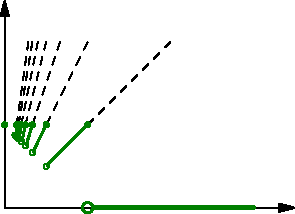
\includegraphics{./Cli02_1.pdf}
 % Cli02_1.pdf: 227x528 pixel, 72dpi, 8.01x18.63 cm, bb=0 0 227 528
 \caption{Exercice \arabic{enumi} : graphe de la fonction}
 \label{fig:Cli02_1}
\end{figure}
